\documentclass[tikz,border=10pt]{standalone}
\usepackage{pgfplots}
\pgfplotsset{compat=newest}
% \pgfplotsset{compat=1.18}
\usepackage[american]{circuitikz}
\usepackage{cmbright}

\definecolor{myred}{RGB}{170,0,0}
\definecolor{myblue}{RGB}{0,0,220}
\definecolor{mygreen}{RGB}{0,150,0}
\definecolor{myorange}{RGB}{255,127,0}
\definecolor{mybrown}{RGB}{150,75,0}

\ctikzset{bipoles/resistor/height=0.2}
\ctikzset{bipoles/resistor/width=0.5}
\ctikzset{bipoles/capacitor/height=0.4}
\ctikzset{bipoles/capacitor/width=0.15}


\begin{document}
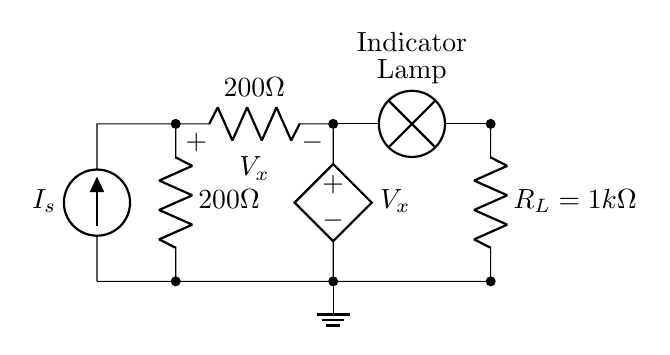
\begin{tikzpicture}
\begin{scope}
    % Define nodes
    \draw (-1.0, 2) node[circ] (O1) {};
    \draw (-1.0, 0) node[circ] (O2) {};
    \draw (1.0, 2) node[circ] (A1) {};
    \draw (1.0, 0) node[circ] (A2) {};
    \draw (3.0, 2) node[circ] (B1) {};
    \draw (3.0, 0) node[circ] (B2) {};

    \draw (-2, 0) 
        to[I, l={$I_s$}] ++(0, 2)
        to (O1) 
        to[R, l=$200\Omega$] (O2)
        -- (-2, 0);
    \draw (O1) 
        to[R, l=$200\Omega$, v_>=$V_x$] (A1)
        to[cV, l^=$V_x$] (A2)
        to (O2);
    \draw (A1) 
        to[lamp, l={\shortstack{Indicator\\Lamp}}] (B1);
    \draw (B1) 
        to[R, l={$R_L=1k\Omega$}] (B2)
        to (A2);
    \draw (A2) node[ground]{};
\end{scope}

\end{tikzpicture}

\end{document}